\documentclass[conference]{IEEEtran}
\IEEEoverridecommandlockouts
\usepackage{cite}
\usepackage{amsmath,amssymb,amsfonts}
\usepackage{graphicx}
\usepackage{textcomp}
\usepackage{xcolor}
\usepackage{booktabs}
\usepackage{placeins}
\usepackage{tikz}
\usetikzlibrary{arrows.meta,positioning,fit,backgrounds,calc}
\usepackage[hidelinks]{hyperref}
\renewcommand{\topfraction}{0.95}
\renewcommand{\dbltopfraction}{0.95}
\renewcommand{\textfraction}{0.05}
\renewcommand{\floatpagefraction}{0.95}
\renewcommand{\dblfloatpagefraction}{0.95}
\setcounter{topnumber}{3}
\setcounter{dbltopnumber}{3}
\setcounter{totalnumber}{5}
\def\BibTeX{{\rm B\kern-.05em{\sc i\kern-.025em b}\kern-.08em T\kern-.1667em\lower.7ex\hbox{E}\kern-.125emX}}

\begin{document}
\title{How Much Fault Tolerance Is in a Fly Brain?\\
{\large Fault-Injection Analysis of a Whole-Connectome Spiking Controller for Physical Intelligence}}

\author{\IEEEauthorblockN{Shuchao Gao}
\IEEEauthorblockA{Waseda University\\
Tokyo, Japan}}

\maketitle

\begin{abstract}
Whole-brain point-neuron models built from complete synaptic wiring diagrams have begun to serve as controllers in embodied settings; fault tolerance has been probed on subnetworks and via targeted silencings but not compared across hardware-motivated fault classes on a whole-brain controller. We take the released leaky integrate-and-fire (LIF) whole-brain model of \emph{Drosophila melanogaster} (138{,}639 neurons, 15.1M signed connections, 54.5M synapse contacts) and inject five hardware-motivated fault classes---weight variability, connection loss, random-unit and hub output silencing, and sensory-channel deafferentation---scoring the population response of descending command neurons. Across 36 fault conditions (12 seeded trials each) under sustained escape-grade drive, the connectome absorbs 50\% lognormal weight variability, retains 76\% of command rate after 50\% connection loss and under 10\% random-unit output silencing, while silencing the top-1\% hubs by total outgoing contact count produces a 2.5$\times$ global over-activity rather than silence. An edge-permuted null preserving weight and degree statistics yields a zero median command rate in every tested condition (no trial reaches the transmission threshold), and relative pathway decay is topology-independent: robustness is consistent with threshold amplification on convergence structure, not graph redundancy alone. We distill the results into five candidate design implications for fault-tolerant neuromorphic controllers.
\end{abstract}

\begin{IEEEkeywords}
neuromorphic computing, connectome, fault tolerance, fault injection, Drosophila
\end{IEEEkeywords}

\section{Introduction}
\label{sec:introduction}
\IEEEPARstart{P}{hysical} intelligence---agents whose perception, decision, and action loops close in the physical world under tight energy and latency budgets---demands controllers that remain robust on imperfect hardware\cite{yuan2026embodiedr,guo2026neurovla}. Neuromorphic systems promise the required efficiency\cite{katti2026neuromorphic,gerven2025neuromorphic}, and spiking implementations on Loihi~2 and FPGA substrates now cover vision and control workloads\cite{wang2025neuromorphic,arfa2025hardwareaware,gautam2025neurocorex}. What remains poorly quantified is how \emph{wiring} determines robustness: engineered spiking networks are designed task-by-task, so their fault tolerance must be re-measured per design\cite{thieu2022effects,yunusoglu2025neuromorphic}. Complete, signed wiring diagrams of whole brains are now public, and point-neuron models built on them reproduce realistic dynamics without training\cite{shiu2024drosophila,lin2024network}; an evolved connectome is thus a field-tested controller and a reference point for engineered fault tolerance.

The released leaky integrate-and-fire (LIF) whole-brain model of \emph{Drosophila melanogaster}\cite{shiu2024drosophila}\footnote{\url{https://github.com/philshiu/Drosophila_brain_model}}, which instantiates the complete FlyWire connectome\cite{lin2024network}, already used targeted computational silencings to identify circuit neurons\cite{shiu2024drosophila}, and we extend that perturbation style into a systematic sweep across \emph{hardware-motivated fault classes}, scored jointly for transmission and activity-envelope compliance. We instrument the visuomotor escape pathway: looming-sensitive visual interneurons (LC4, LPLC2) converge onto descending command neurons (DNp01, DNa02, DNp04, DNb01) whose activation evokes take-off and escape steering\cite{simpson2023descending}. Its failure modes map directly onto hardware fault classes: weight imprecision, broken interconnect, dead cores, dead sensors.

We inject five fault families (Section~III-C), each over 12 seeded 600\,ms trials, with two controls: an edge-permuted null preserving weights and degree statistics, and an analytic pathway-mass computation. Our contributions: (i) a fault-injection framework mapping hardware failure modes onto a connectome-constrained 138k-neuron LIF model; and (ii) the first tolerance curves of descending-neuron output in a complete connectome (50\% weight noise absorbed, 50\% connection loss retains 76\%, 10\% unit loss leaves the median unchanged): top-1\% hub loss instead produces a $2.5\times$ \emph{activity runaway} that passes transmission while violating the output envelope, and whole-channel deafferentation is the only catastrophic mode. We further (iii) decompose why graph redundancy alone explains neither specificity nor graceful degradation (threshold amplification as a candidate account) and (iv) distill five candidate design implications for fault-tolerant controllers.

\section{Related Work}
The release of complete wiring diagrams for the adult \emph{Drosophila} brain\cite{lin2024network} has shifted connectome research from static graph analysis to executable models: visual-system convolutions\cite{liew2026connectomebased}, neuron-level response prediction\cite{xie2025visual}, learned tasks and whole-body locomotion on whole-CNS wiring\cite{cho2026drosophila,senge2026connectome,jin2026wholebrain}, biofidelic processing units\cite{yu2025biological}, and descending-neuron input sharing\cite{zhang2026synaptic,drummond2026population}. Closest to our substrate, the released LIF whole-brain model (footnote 1) reproduces global activity and has been ported to Loihi~2\cite{wang2025neuromorphic}. Lesion studies now perturb whole connectomes---amyloid-like pathology on a fly CNS graph\cite{jo2026simulating}, function-preserving sparsification of the \emph{Drosophila} model\cite{an2026sparse}, and deletion of critical nodes from an SNN sugar-sensing subnetwork scored by a sensory rate threshold\cite{adler2026latent}---but none sweeps hardware-motivated fault classes on a fixed whole-brain controller or separates output transmission from activity-envelope compliance; we do both.

Graph-theoretic lesion studies score the structural attack tolerance of brain networks\cite{aerts2016brain}, not dynamics; spiking-network weight-noise robustness is mostly characterized on small trained architectures\cite{thieu2022effects,yunusoglu2025neuromorphic}, with adaptive mitigation now studied at the edge\cite{luca2026learned}; purpose-built fault-injection frameworks for trained SNNs---SpikeFI\cite{spyrou2024spikefi}, SpikingJET\cite{gogebakan2024spikingjet}---automate this but score task accuracy on human-designed networks, with follow-up work on STDP-trained robustness and population-coded redundancy\cite{jouni2025stdptrained,gleyo2026population}. Hardware platforms expose complementary constraints: on-chip variability co-design\cite{arfa2025hardwareaware}, FPGA precision--capacity trade-offs\cite{gautam2025neurocorex}, permanent interconnect faults\cite{chessa2026crosslayer}, and trained-CNN dependability\cite{graciamorn2026dependability}. Insect-inspired collision-aversion circuits are robust by construction but small and hand-designed\cite{shuang2023opplod}, and fault-injection benchmarking of neuromorphic systems is only beginning\cite{yik2023neurobench,medvedeva2025formalizing}; a complete connectome enables it at the scale of an entire evolved controller.

\section{Fault-Injection Framework}
\subsection{Whole-Brain Spiking Substrate}
We adopt the released whole-brain LIF model of \emph{Drosophila}\cite{shiu2024drosophila} (Section~\ref{sec:introduction}), implemented in Brian2\cite{goodman2009brian} and built on the FlyWire connectome\cite{lin2024network}. Every neuron is a current-based LIF unit (threshold $-45$\,mV, reset $-52$\,mV, membrane time constant 20\,ms, refractory 2.2\,ms, axonal delay 1.8\,ms). Each connection in the released table becomes a delta-conductance synapse whose jump is $0.275$\,mV per counted contact and decays with a 5\,ms synaptic time constant, signed by the presynaptic cell's neurotransmitter; the table yields 15{,}091{,}983 connections between 138{,}639 neurons (54.5M contacts), 40\% inhibitory. As in the released model, baseline firing is zero: the only external input is the stimulus Poisson group over the driven set, so every recorded spike traces back to the stimulated cells. Our engine restores the full network state at the start of every trial, so all conditions share identical initial states, while the stimulus draws a fresh realization each trial: reported dispersion includes stimulus variability. One 600\,ms trial runs in ${\approx}3.5$\,s on one CPU core.

\subsection{Task: Visuomotor Escape}
The instrumented pathway (Fig.~\ref{fig:system}) is the fly's looming-triggered escape circuit: looming-sensitive visual projection neurons LC4 (104) and LPLC2 (210) converge on descending neurons\cite{shuang2023opplod,simpson2023descending}. Because collision-sensing models treat looming as sustained high-rate drive, we drive the sensory cells---and, as a control, an equal-sized random set---with independent 150\,Hz Poisson trains gated per trial, rather than modeling looming kinetics. The primary readout is the population rate of the command set \{DNp01, DNa02, DNp04, DNb01\} (8 neurons); all 1{,}299 descending neurons serve as a secondary readout. Calibration drove the command population to $94.6$\,Hz (interdecile 93.6--95.8\,Hz, first-spike latency 4.4\,ms; 10-trial set) under escape stimulation but only 8.2\,Hz (6.4--9.2\,Hz) under random stimulation; $\theta=51.4$\,Hz (the 94.6/8.2\,Hz midpoint), every pass/fail classification below is unchanged for thresholds between the observed trial extremes (9.2--63.1\,Hz); Section~IV uses the 12 sweep trials.

\begin{figure}[tb]
\centering
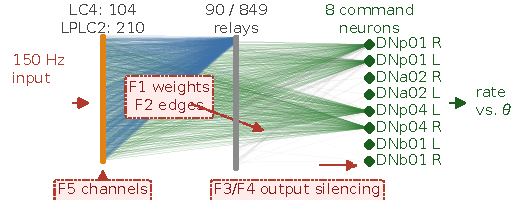
\includegraphics[width=0.96\columnwidth]{figs/fig0_pathway.pdf}
\caption{The instrumented escape pathway, drawn from the connectome itself. Left: the 314 driven sensory cells (LC4, LPLC2); center: the 90 top-ranked of 849 two-hop relays; right: the 8 command DNs. Line width and opacity scale with synapse count (594 direct sensory$\to$DN edges); dashed red marks the fault-injection points (F5 channels; F1/F2 synapses; F3/F4 units). Inset: reconstructed adult brain, adapted from Dorkenwald et al.\cite{dorkenwald2024neuronal} (CC~BY~4.0).}
\label{fig:system}
\end{figure}

\subsection{Fault Taxonomy}
Five fault families cover the hardware-relevant failure modes. F1 multiplies every synaptic weight by an i.i.d.\ mean-preserving lognormal factor ($\sigma\in\{0.05,0.1,0.2,0.5\}$), modeling analog weight variability and bit-level imprecision. F2 deletes a random fraction $f\in\{0.05,0.10,0.25,0.50\}$ of synapses, modeling interconnect or memristor failures. F3 silences all output synapses of a random fraction $f\in\{0.01,0.02,0.05,0.10\}$ of units, excluding input and readout cells (unit removal in this delta-synapse model), modeling dead cores. F4 applies the same operation to the top 1\%, 2\%, or 5\% of units ranked by total outgoing synapse count (again excluding input and readout), modeling failure of high-fanout components; these cells carry 9--22\% of all connections (1\%, 2\% and 5\% sets, respectively), a targeted, correlated version of F3. F5 zeroes all outgoing synapses of one (LC4 or LPLC2) or both sensory channels, modeling sensor or afferent-path failure. All faults are applied after state restoration; F4 and F5 act on fixed cell sets, while F1--F3 redraw their realization each trial from SHA-256 seeds over (phase, condition, trial)---12 independent draws per condition, exactly reproducible from the archived seeds (the stimulus stream is not re-seeded, so re-runs are statistically equivalent rather than bit-identical).\footnote{Code, connectome-derived edge lists, and per-trial records: \url{https://github.com/Scophield/drosophila-fault-injection}.}

\subsection{Controls}
Two controls isolate what the biological wiring contributes. The first is an edge-permuted null: every synapse keeps its presynaptic partner, weight, and sign, but its postsynaptic target is randomly reassigned. This preserves out-degrees, weights, and the global in-degree histogram while destroying which inputs converge onto each target---and with them all multi-hop structure; the identical sweep runs on it. The second is analytic: for both graphs we compute the \emph{pathway mass} $m_k=\mathbf{1}_{\mathrm{DN}}^{\top}A^{k}\mathbf{1}_{\mathrm{in}}$, the synapse-weighted total of all $k$-hop directed paths from LC4$\cup$LPLC2 into the full descending layer ($A$ holds contact counts, i.e., absolute signed strengths; $m_k$ counts $k$-step walks of either sign---a wiring-density proxy, not signal flow), on the intact graph and after the F2 deletion levels; comparing its decay with the output decay separates topological redundancy from dynamical amplification.


\section{Results}
\subsection{Baseline: The Connectome Is a Specific, Low-Latency Controller}
Driving LC4 and LPLC2 at 150\,Hz produces a command-population rate of $94.7$\,Hz (median over 12 trials; interdecile 94.0--95.6\,Hz) with 4.05\,ms median first-spike latency, far above $\theta$ (Fig.~\ref{fig:baseline}). An equal-sized random set, driven identically, yields only $8.2$\,Hz on the same readout while producing \emph{more} total activity (293k vs.\ 40k spikes): the readout is pathway-specific, not generic arousal. When both sensory channels are silenced (F5\textsubscript{both}), the command rate collapses to exactly zero in every trial while the rest of the brain keeps spiking at background level: the score measures transmission through the instrumented pathway.

\begin{figure}[tb]
\centering
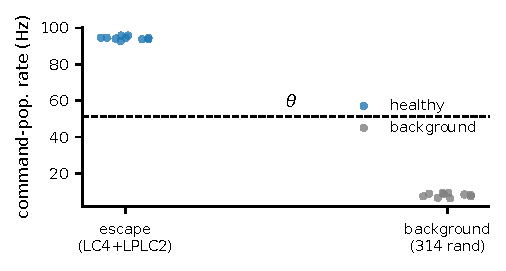
\includegraphics[width=\columnwidth]{figs/fig2_baseline.pdf}
\caption{Readout specificity. Command-population rate under escape stimulation (LC4$+$LPLC2) versus matched random-site stimulation (314 cells); dashed line: $\theta$.}
\label{fig:baseline}
\end{figure}

\subsection{Tolerance Curves: Noise Is Absorbed, Disconnection Degrades Gracefully}
Figure~\ref{fig:curves} shows dose--response curves for the two most consequential families; the F1 and F3 responses are flat in median (Table~\ref{tab:principles}). Weight variability (F1) leaves the median unchanged: at $\sigma{=}0.5$ the rate is $94.2$\,Hz (healthy: 94.7\,Hz) while the trial dispersion widens (interdecile 90.4--100.8 vs.\ 94.0--95.6\,Hz healthy), and total activity rises only from 39.7k to 41.6k spikes. Random synapse deletion (F2) degrades gracefully: 5\% and 10\% loss leave the rate at 91.9 and 93.1\,Hz, 25\% loss retains $84.5$\,Hz (89.2\% of baseline), and even 50\% loss retains $72.4$\,Hz (76.5\%), with all 12 trials passing the transmission criterion in every condition (weakest trials 63.1 and 68.1\,Hz---above $\theta$ by $\geq$22\%). Disconnection's cost appears predominantly in latency: 4.05 to 5.4\,ms at 50\% loss (+33\%), consistent with recruitment of longer residual multi-hop routes; which dominates a task-level error budget is workload-dependent. Random unit loss (F3) up to 10\%---nearly 14{,}000 neurons with all their synapses---leaves the median unchanged (95.1 vs.\ 94.7\,Hz): command drive integrates over hundreds of converging populations, and no tested random 10\% slice is load-bearing. The wide 1{,}299-neuron descending layer tracks the same pattern (2{,}941 spikes healthy vs.\ 1{,}918 at 50\% loss), so the graded response is a property of command encoding, not of the eight-neuron readout.

\begin{figure*}[tb]
\centering
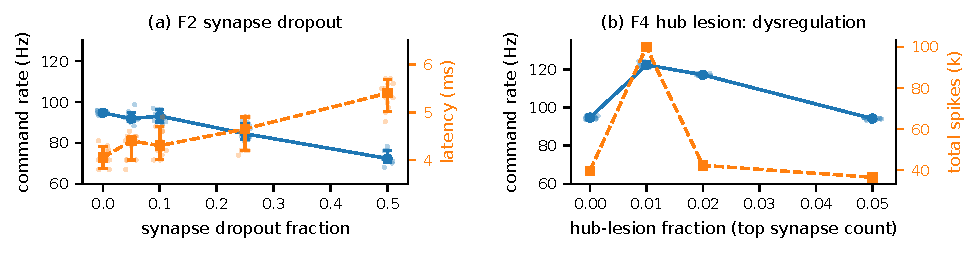
\includegraphics[width=\textwidth]{figs/fig3_curves.pdf}
\caption{Behavioral tolerance curves (medians over 12 trials, blue: rate; orange: latency ms (a) / total spikes (b); dots: trials; dotted grey: healthy medians). (a) Synapse dropout: 76\% of the command rate retained at 50\% loss while latency rises 33\%. (b) Hub lesion: dysregulation, not signal loss.}
\label{fig:curves}
\end{figure*}

\begin{figure*}[tb]
\centering
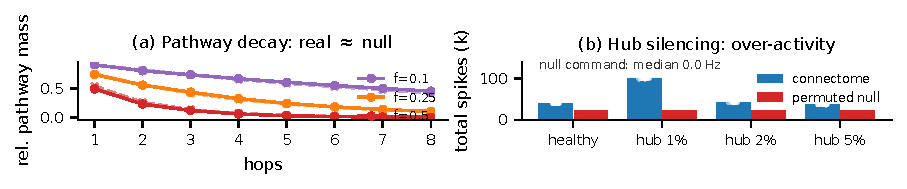
\includegraphics[width=\textwidth]{figs/fig4_topology.pdf}
\caption{Topology contrast. (a) Route mass under edge loss, normalized per graph (solid: connectome, dashed: permuted null): relative decay nearly identical, absolute mass 5.8--17.7$\times$ higher. (b) Activity under hub lesions: runaway only in biological wiring; null command readout at 0.0\,Hz.}
\label{fig:topology}
\end{figure*}

\subsection{Hub Loss Produces Runaway, Not Silence}
The dose--response of hub removal (F4) is non-monotonic and qualitatively different from every distributed fault (Figs.~\ref{fig:curves}b, \ref{fig:topology}b). Removing the top 1\% of cells ranked by total outgoing synapse count (1{,}386 neurons, 9.1\% of all connections) \emph{increases} the command rate to $122.3$\,Hz (+29\%, interdecile 121.1--123.9\,Hz across trials) and more than doubles global activity (99.9k spikes, $2.52\times$ healthy; Mann--Whitney vs.\ healthy $p<10^{-4}$, as for F2$_{50}$ and F5$_{\mathrm{both}}$); at 2\% the rate stays elevated (117.1\,Hz) with activity partially normalized (42.4k); at 5\% (22.4\% of connections) both metrics return to near-baseline (94.2\,Hz, 36.4k). A matched-scale contrast shows this is not a size effect: random 10\% unit ablation disconnects 10.0\% of connections (more than the hub set's 9.1\%) yet leaves the readout unchanged (95.1\,Hz). Hub lesions do not starve the pathway of drive---they remove broadly connected inhibitory regulation, and spared circuitry over-drives the command layer: about 62\% of removed hub output connections are inhibitory, versus 40\% network-wide. We therefore score \emph{transmission} (rate $\geq\theta$) and an \emph{activity envelope} (rate and total activity within $2\times$ of healthy) separately: hub loss at 1\% passes transmission in all trials while violating the envelope in all 12 (the violation persists for any envelope multiplier between $1.5\times$ and $2\times$); every distributed fault passes both; F5\textsubscript{both} fails both. The envelope violation is the engineered system's dangerous mode: output exceeds its envelope while every per-unit monitor reads ``active.'' The same lesion in the permuted null produces no such signature, tying the runaway to biological hub structure, not degree heterogeneity per se.

\subsection{What the Wiring Contributes: Null Network and Pathway Analysis}
The permuted null dissociates specificity from redundancy: out-degrees, weights, and the in-degree histogram survive, convergence is reassigned, and the null transmits \emph{nothing} to the command layer (0.0\,Hz in every condition and trial); its broad 1{,}299-neuron readout falls to background (45.5 spikes per trial vs.\ 2{,}941 healthy) and global activity to about 60\% of the biological level (23.8k vs.\ 39.7k)---it spikes, but nothing converges onto descending output. Pathway mass quantifies the convergence advantage: 5.8$\times$ more 1-hop and 17.7$\times$ more 4-hop route mass from sensory input into the descending layer than the null. Yet \emph{relative} pathway-mass decay under the same deletion levels is nearly identical in both graphs (at $f{=}0.5$, $k{=}8$: 0.3\% vs.\ 0.4\% of baseline; Fig.~\ref{fig:topology}a). Combined with behavior degrading far more slowly than pathway mass (76\% functional retention at $f{=}0.5$ against 5.8\% four-hop route mass), this rules out graph redundancy alone and is consistent with a threshold-amplification account of the topological-to-functional conversion. The comparison does not isolate the dynamics by itself: the 594 direct sensory$\to$DN connections, which survive edge deletion in proportion, and excitation--inhibition rebalancing could contribute; targeted controls are needed. A threshold-amplification account is simple: with $N$ afferents converging and per-synapse survival $p$, converged drive scales as $Np$ while $k$-hop route mass decays as $p^k$ (6.25\% at $k{=}4$, $p{=}0.5$); the threshold's saturating nonlinearity maps drive onto output, so the rate retains 76.5\% at $p{=}0.5$ and 89.2\% at $p{=}0.75$, above the linear 50\% and 75\% bounds the account predicts; near-threshold drive is where it should fail, saturation compressing increases more than decreases. Graceful degradation here reflects convergent wiring preserving aggregate drive plus threshold dynamics compressing drive changes into small rate changes.


\section{Candidate Design Implications for Embodied Neuromorphic Controllers}
\label{sec:implications}
Three of the five implications concern where redundancy pays. Because $50\%$ weight variability and $10\%$ unit-output silencing leave the median command rate unchanged (99.4\% and 100.4\% of baseline), precision and per-unit yield can be traded against wiring redundancy: weights may drift by a lognormal $\sigma$ of 0.5---beyond most analog or multi-bit resistive devices---and 10\% of cores may fail outright, provided many routes converge\cite{arfa2025hardwareaware,thieu2022effects}. Disconnection is paid in latency, not rate---$76.5\%$ of the rate survives at $50\%$ loss while latency rises $33\%$---so a real-time loop should budget that curve (Fig.~\ref{fig:curves}a).

The other two implications concern failure modes that per-unit monitoring misses. Hub silencing is the only class that can \emph{amplify}, and its sign matters more than its size: removing the inhibitory half of the top 1\% raises activity $21\times$, while the full set hides this behind a matching excitatory loss---so monitor the activity envelope, not liveness; and since 8.6\% of inhibitory mass removed at random was benign in eleven of twelve trials while 5.6\% removed at hubs always destabilised, sparing high-fanout \emph{inhibitory} units is the cheaper mitigation. Deafferentation is the opposite extreme: either channel alone retains 68--79\% of the median rate, but losing both drives the pathway to zero, making the sensor interface---not the synaptic fabric---the first redundancy candidate. Because relative pathway decay is identical while only the biological graph yields a decodable command, fault injection belongs pre-deployment\cite{yik2023neurobench,medvedeva2025formalizing}.

\enlargethispage{3\baselineskip}
\section{Limitations and Conclusion}
Our LIF abstraction fixes one drive rate, the hub sign split is measured at that one rate, and correlated damage is excluded. One pathway is instrumented, so the ordering is a hypothesis for others rather than a whole-brain law, and its vulnerability to aging\cite{gaitanidis2025drosophila} suggests tolerance is not fixed either. Under the tested drive the median rate survives weight noise and unit silencing, retaining 76.5\% at 50\% loss; the dangerous failure is inhibitory-hub over-activity, which a closed loop turns into lost steering.


\bibliographystyle{IEEEtran}
\bibliography{refs}

\end{document}
